\documentclass[12pt,a4paper,twoside]{article}

% LaTeX-Umsetzung der "Richtlinien f�r Projekt- und Diplomarbeiten"
% der LFE Medieninformatik, LMU M�nchen. (Autor: Richard Atterer, 27.9.2006, 23.10.2007), Bug-Fixing Mark Kaczkowski (23.6.2008)

\usepackage[T1]{fontenc} % sonst geht \hyphenation nicht mit Umlauten
\usepackage[latin1]{inputenc} % man kann schreiben ����, statt "a"o"u"s
%\usepackage[utf8]{inputenc} % wie oben, aber UTF-8 als Encoding statt ISO-8859-1 (latin1)
\usepackage[ngerman,english]{babel} % deutsche Trennregeln, "Inhaltsverzeichnis" etc.
%\usepackage{ngerman} % Alternative zum Babel-Paket oben
\usepackage{mathptmx} % Times-Roman-Schrift (auch f�r mathematische Formeln)

% Zum Setzen von URLs
\usepackage{color}
%\definecolor{black}{rgb}{0,0,0}
\usepackage[plainpages=false,bookmarks=true,bookmarksopen=true,colorlinks=true,
  linkcolor=black,citecolor=black,filecolor=black,
  menucolor=black,urlcolor=black]{hyperref}

% pdflatex: Bilder in den Formaten .jpeg, .png und .pdf
% latex: Bilder im .eps-Format
\usepackage{graphicx}

\usepackage{fancyhdr} % Positionierung der Seitenzahlen
\fancyhead[LE,RO,LO,RE]{}
\fancyfoot[CE,CO,RE,LO]{}
\fancyfoot[LE,RO]{\Roman{page}}
\renewcommand{\headrulewidth}{0pt}
\setlength{\headheight}{14.5pt} % behebt headheight Warning

% Korrektes Format f�r Nummerierung von Abbildungen (figure) und
% Tabellen (table): <Kapitelnummer>.<Abbildungsnummer>
\makeatletter
\@addtoreset{figure}{section}
\renewcommand{\thefigure}{\thesection.\arabic{figure}}
\@addtoreset{table}{section}
\renewcommand{\thetable}{\thesection.\arabic{table}}
\makeatother

\sloppy % Damit LaTeX nicht so viel �ber "overfull hbox" u.�. meckert

% R�nder
\addtolength{\topmargin}{-16mm}
\setlength{\oddsidemargin}{25mm}
\setlength{\evensidemargin}{35mm}
\addtolength{\oddsidemargin}{-1in}
\addtolength{\evensidemargin}{-1in}
\setlength{\textwidth}{15cm}
\addtolength{\textheight}{34mm}
%______________________________________________________________________

\begin{document}

\pagestyle{empty} % Vorerst keine Seitenzahlen
\pagenumbering{alph} % Unsichtbare alphabetische Nummerierung

\begin{center}
\textsc{Ludwig-Maximilians-Universit�t Munich}\\
Department of Computer Science\\
Database Systems Group\\
Prof.\ Dr.\ Thomas Seidl

\vspace{5cm}
{\large\textbf{Bachelor's Thesis}}\vspace{.5cm}

{\LARGE An even longer Title to see how it looks when using two lines in the document}\vspace{1cm}

{\large Rainer Wittmann}\\
Matriculation Number: 10954724\\
\href{mailto:r-wittmann@outlook.de}{r-wittmann@outlook.de}

\end{center}
\vfill

\begin{tabular}{ll}
Supervised by: & Gregor Joss�\\
& PD Dr. Matthias Schubert\\
Submitted on: & \today
\end{tabular}
%______________________________________________________________________

\selectlanguage{english}
\clearpage
\section*{Definition of Task}
\label{Definition of Task}

Definition of Task

\vfill % Sorgt daf�r, dass das Folgende an das Seitenende rutscht

\noindent I confirm that I independently prepared the thesis and that I used only the references and auxiliary means indicated in the thesis.

\bigskip\noindent Unterhaching, \today

\vspace{4ex}\noindent\makebox[7cm]{\dotfill}

%______________________________________________________________________

\cleardoublepage
\pagestyle{fancy}
\pagenumbering{roman} % R�mische Seitenzahlen
\setcounter{page}{1}

% Inhaltsverzeichnis erzeugen
\tableofcontents

%\setlength\parskip{\baselineskip}

%______________________________________________________________________

\cleardoublepage

% Arabische Seitenzahlen
\pagenumbering{arabic}
\setcounter{page}{1}
% Ge�ndertes Format f�r Seitenr�nder, arabische Seitenzahlen
\fancyhead[LE,RO]{\rightmark}
\fancyhead[LO,RE]{\leftmark}
\fancyfoot[LE,RO]{\thepage}

%______________________________________________________________________

% Der Befehl \cleardoublepage erscheint nur vor \section, nicht vor
% den "kleineren" Gliederungsbefehlen wie \subsection!
%\cleardoublepage % Neue rechte Seite anfangen
%\section{State of the Art}

%\begin{figure}%[btph]
  %% Datei ``beispielbild.eps'' oder ``beispielbild.png'', zentriert
  %\begin{center}\includegraphics{beispielbild}\end{center}

  %% Datei auf 8cm Breite verkleinert/vergr��ert
  %\includegraphics[width=8cm]{beispielbild}
  %% Datei auf ganze Breite des Texts vergr��ert
  %\includegraphics[width=\columnwidth]{beispielbild}
  %% Datei auf 60% der Textbreite verkleinert/vergr��ert
  %\includegraphics[width=.6\columnwidth]{beispielbild}
  %% Weitere Optionen (Ausschnitt, drehen etc.) in der Doku zum graphicx-Paket

 % \begin{center}\LARGE [BILD]\end{center}
  %\caption{Bildunterschrift}
  %\label{fig:beispielbild}
%\end{figure}

%\bigskip % Gr��erer Abstand zum vorherigen Absatz

%\begin{description}
%  \item[Medienwirkung:] Ein Spezialfach der Kommunikationswissenschaft. F�r das erfolgreiche Studium des Anwendungsfachs Mediengestaltung ist eine k�nstlerische Begabung erforderlich.
%  \item[Medienwirtschaft:] Ein Spezialfach der Betriebswirtschaftslehre
%  \item[Mediengestaltung:] Ein Spezialfach der Kunstwissenschaft
%\end{description}

%\subsubsection{Was Sie schon immer wissen wollten, aber nie zu fragen
%  wagten}

%\paragraph{�berschrift}
%Diese �berschrift erscheint fettgedruckt am Anfang des Absatzes.

%\subsubsection{Was Sie nicht wissen wollten}

%Text text textextext\footnote{Oder so �hnlich}.

%\_____________________________________________________________________

\section{Introduction}
\label{sec:Introduction}

%Introduction to the problem, motivation, approaches, goals

%The developed project can be viewed at https://r-wittmann.github.io/mario. Furthermore the code of the project can be cloned from my git repository at https://github.com/r-wittmann/mario for analysis and further development.

One big part of the theoretical and practical work done by the Database Systems Group (DBS) regards graph data and algorithms that solve problems on graphs in particular search for shortest paths from one node to another. The algorithms which are solving this issue, like Dijkstra and A-Star for example, are constantly refined to perform faster, less error prune and more precise and also find use in other algorithms to solve more complicated tasks. In 2011 the Multi Attribute Routing in Open Street Map Project (MARiO) \cite{MARiO11}, was initiated to further enhance the development process, the implementation and the visualisation of new or updated algorithms and methodologies.

"MARiO is an open source project combining functionalities for data integration and preprocessing, implementation of new algorithms and performance evaluation" \cite{MARiO11}. It was developed in Java 1.6 and follows a plugin architecture, i.e. allows the implementation of new algorithms without the need to alter the original code base. What seemed to be a great technology at the time, MARiO is now outdated, takes extensive amounts of time to download, compile and start on a local machine and doesn't follow any kind of modern software design pattern. Further information about MARiO will be given in section \ref{sec:Description of the Backend}.\medskip

The task of this bachelor's thesis was the development of a modern browser application constituting as a visualisation of the in parallel implemented back end server at the DBS. This type of architecture is called server-client architecture which separates the representation on client side from the processing and storing of large amounts of data and the implementation of algorithms on the server side. Implementing the back end was not part of this thesis.

The front end, developed in AngularJS for large browser and platform compatibility, 

%\_____________________________________________________________________

\cleardoublepage 
\section{State of the Art v}
\label{sec:State of the Art}

As the software developed in the course of this thesis depends on various frameworks, specifications and other projects, this section will illustrate and delimit the underlying technologies used. First an overview of AngularJS, a JavaScript framework for dynamic views, is given, which is followed by an introduction to to the Leaflet project for mapping applications. The third section covers GeoJson as a standard for geospatial data and finally the HERE-API for map imagery and additional map data will be introduced.

%\____ AngularJS

\subsection{AngularJS v}
\label{subsec:AngularJS}

When one is implementing a web application, HTML, CSS and JavaScript are most commonly the technologies of choice. HTML is great for declaring static documents and CSS for styling, but both lack the ability to react to dynamic changes of values and views and are hence not up to the challenges of a modern web application. As HTML and CSS are rather old technologies various developers generated a multitude of ways to compensate said shortcomings and JavaScript was one of them. Developed in 1995 by Netscape employee Brendan Eich, JavaScript has been in a continuos development process, is now implemented in all modern web browsers without the need for plugins and almost all websites depend on it. JavaScript is standardised by Ecma International in the latest ECMA-262 language specification \cite{ECMA}. 

But still there was room for improvement. In the past few years with web 2.0, excessive use of mobile browsers and the resulting higher user interaction with websites, additional functionalities were needed and developed. But non of these frameworks addressed the basic problem with HTML, namely that it was not designed for dynamic views. AngularJS on the other hand extends the existing HTML vocabulary and allows for expressive, readable and quick to develop code. Based on HTML and JavaScript, AngularJS is a framework which allows developers to have full access to standard syntax and facilitates the dynamization of web applications.

Normally when a user visits a website, the HTML template is requested from the server and loaded into the web browser, including CSS for styling and all JavaScript files needed for the utilisation of the website. AngularJS applications differ from that process. In the bootstrapping phase, which is started right after the HTML markup is loaded, the core AngularJS functionalities are merged with the template to provide basic features. After the AngularJS code is available in the web browser, the module referenced from the HTML template is generated and all dependencies are injected into and made available to this module. Also the scope is introduced to the application allowing the initially generated static view to be replaced by AngularJS's dynamic view.\medskip

AngularJS is based on the Model View Controller pattern (MVC) which allows for a strict separation of the underlying data structure, the View, which is displayed to the user and the controllers, implementing needed business logic. As the so called scope, which is used as the model, is accessible from both view and controller, it binds both components together. Each AngularJS application has exactly one root scope which may have several child scopes as every directory creates its own scope. The child scopes inherit from their parent prototypically. Controllers can use services, factories and providers for additional functionalities which are part of the above mentioned dependencies injected into the controller.

The ability to bind view elements to variables and functions on the scope and vice versa is called two way data binding and is one of the main reasons AngularJS is favoured over many other frameworks. All changes to the view, for example via input fields, are immediately reflected to the scope and all changes to variables on the scope are propagated to the view keeping them both up to date. All functions stored on the scope are accessible from the view elements allowing for easy and fast implementation of click listeners and other business logic.\medskip

As JavaScript is an untyped language, which means that variables don't have to be declared as one particular type, the developer receives almost no errors while compiling the code and therefore often stand before the problem of finding errors himself. AngularJS has built in features for testing to simplify the process. Two basic concepts of testing, unit tests and end-to-end tests, will be explained in the following two paragraphs.

Unit tests are about testing small units of code without building the whole project around it. This ensures locating errors exactly were they occur and minimise the risk of cross contamination between modules and controllers. Karma and Jasmine are two favoured tools for unit testing in AngularJS applications. Both tools are easy to use and allow for structured tests of small units of code. Especially Jasmin makes it easy for the developer to write readable code which is easy to understand and maintain.

Once an application becomes bigger, manual unit testing becomes more and more work and is no longer recommended. Additionally some issues may occur when integrating components or resulting from interplay of more than one module. At this point the developer has to think about end to end testing which can be executed automatically. The recommended tool for end-to-end testing is called Protractor which, using the same syntax as Jasmine, allow for browser testing and the simulation of user interaction.\medskip

For this application AngularJS version 1.5.5 was used as Angular 2 was not at a stable release at the beginning of this project. AngularJS is mainly maintained by Google and by a community of individuals and cooperations which contribute to the open source project. 

%\____ LeafletJS

\subsection{Leaflet v}
\label{subsec:Leaflet}

The goal of this thesis was to enable users to request routes using various algorithms and methodologies implemented on the server at DBS and display the servers response on client side. For this purpose a mapping framework was needed to handle all issues regarding the download of map tile imagery, user interaction and overlay handling. The API for requesting map imagery will be described in \ref{subsec:HERE API}.

"Web based mapping has evolved rapidly over the last two decades, from MapQuest and Google to real-time location information on our phones' mapping apps" \cite{Crickard14}. Consequently various alternatives are available for mapping applications. After evaluating the possibilities Leaflet stood out for its light weight of about 33 kB of JavaScript, the compatibility to almost all platforms, the vast amount of third party plugins and the simplicity, usability and performance of the API. 

Other projects and products under consideration were, for example, MapBox and the Google Maps API. MapBox is a company offering lots of services such as designing and hosting of maps, geocoding, routing and many more. Unfortunately the terms of use are rather complex and restricting. 2013 MapBox and Leaflet joined forces and MapBox is now using Leaflet for their front end integrations \cite{MacWright13}. These were the main reasons MapBox was not chosen for this project. The Google Maps API is even more restrictive than MapBox. Only Goggle Maps imagery can be used with the API and it is not allowed to display third party information, such as the calculated routes from the server of this project, which rendered it unusable for this development.\medskip

This paragraph will summarise the history of Leaflet. After discovering the complexity and bulkiness of then industry standard for mapping, OpenLayers, in 2008, Vladimir Agafonkin decided to implement a simple, lightweight mapping library. Against resistance of his superiors at Cloud Made, his employer at the time, and criticism from the community of map developers, he succeeded in developing the now most commonly used framework for mapping applications \cite{Agafonkin15}. Since the initial release of Leaflet in May 2011 with limited functionalities and without the support for major open standards, such as the Web Map Service (WMS) \cite{WMS} and the Web Feature Service (WFS) \cite{WFS} the framework has matured considerably. As the second release candidate 1.0-rc2 is out of development, major version update 1.0 is soon to be deployed with even more features and improved mobile friendliness.

For the development of this project the most recent stable Leaflet version 0.7.7 (published October 26, 2015) was used. Leaflet is maintained by now MapBox employee and original Leaflet creator Vladimir Agafonkin who is heavily supported by a large base of contributors and benefits from vast amounts of developers implementing third party plugins.\medskip

To leverage the combination of the power of AngularJS and the simplicity of Leaflet the Angular-Leaflet-Directive (ALD), developed by David Rubert (tombatossals) was introduced to this project for easy integration of Leaflet and bi-directional binding between the map and AngularJS's scope. With the ALD it is possible to include a Leaflet map with just one line of HTML code.

ALD version 0.9.0 was used for this project. It is still maintained by the original creator David Rubert with major help from the AngularUI project.

%\____ GeoJson

\subsection{GeoJson}
\label{subsec:GeoJson}

GeoJson as a information standard, compare to different Json format for geospatial data.

GeoJSON is a format for encoding data about geographic features using JavaScript Object Notation (JSON) [RFC7159]. Geographic features need not be physical things; any thing with properties that are bounded in space may be considered a feature. GeoJSON provides a means of representing both the properties and spatial extent of features.

The GeoJSON format specification was published at http://geojson.org in 2008. GeoJSON today plays an important and growing role in many spatial databases, web APIs, and open data platforms. Consequently the implementers increasingly demand formal standardisation, improvements in the specification, guidance on extensibility, and the means to utilize larger GeoJSON datasets.

%\____ HERE API

\subsection{HERE API}
\label{subsec:HERE API}

Description of the HERE API, problems, features, limitations. (Legal matters in 4.3)


%\_____________________________________________________________________

\cleardoublepage
\section{Description of the Backend}
\label{sec:Description of the Backend}

Introduction to the Description of the Backend section, move from complete Java project to an only server application which can be contacted via Rest Services.

%\____ Backend Functionalites

\subsection{Backend Functionalities}
\label{subsec:Backend Functionalities}

Summarise the implemented functionalities and algorithms from various papers, provided by Gregor. 

\paragraph{functionality/algorithm I} description of functionality/algorithm I
\paragraph{functionality/algorithm II} description of functionality/algorithm II
\paragraph{functionality/algorithm III} description of functionality/algorithm III

%\____ Rest API

\subsection{Rest API}
\label{subsec:Rest API}

Implemented Rest contact points, how to contact, performance

%\_____________________________________________________________________

\cleardoublepage
\section{Development of the Front End}
\label{sec:Development of the Front End}

Introduction to my working process, development etc.

%\____ Build Tools and Frameworks for Development

\subsection{Build Tools and Frameworks for Development}
\label{subsec:Build Tools and Frameworks for Development}

Software development nowadays depends on various frameworks, other projects and build tools. These will be explained and described in this subsection.

%\____ git and GitHub-Pages

\paragraph{git and GitHub-Pages}

git as version control, comparison to other/older version control systems. GitHub-Pages to deliver the homepage even if its not the usual way of doing it.

%\____ npm and bower

\paragraph{npm and bower}

nodes npm as dependency manager for all development dependencies, bower for all dependencies needed for the front end to be displayed

%\____ Agile Software Development

\paragraph{Agile Software Development}

Agile in general, Scrum, my development process

%\____ Implemented Features

\subsection{Implemented Application}
\label{subsec:Implemented Application}

\begin{figure}
  \begin{center}
    \includegraphics[width=0.95\columnwidth]{resources/classdiagram.png}
  \end{center}
  \caption{Class diagram of the application}
  \label{fig:appclassdiagram}
\end{figure}

figure \ref{fig:appclassdiagram}

\subsection{Implemented Features v}
\label{subsec:Implemented Features}

This subsection will contain all implemented features, describe them from a usability and technical standpoint and uncover shortcomings which will be an essential part of chapter \ref{sec:recap}. The original features this thesis was constructed for, namely the calculation of routes using various algorithms and the calculation of intermodal routes including public transportation will be explained in \ref{subsubsec:Route Calculations} and \ref{subsubsec:Intermodal Route Calculations}. The remaining features are the points of interest search (see \ref{subsubsec:Points of Interest}), geocoding addresses (see \ref{subsubsec:Geocoding Addresses}) and the animated display of simulations of cars and thunderstorms which are the result of another students bachelors thesis (see \ref{subsubsec:Simulation}) (zitieren).

%\____ Points of Interest

\subsubsection{Points of Interest v}
\label{subsubsec:Points of Interest}

\begin{figure}
  \begin{center}
    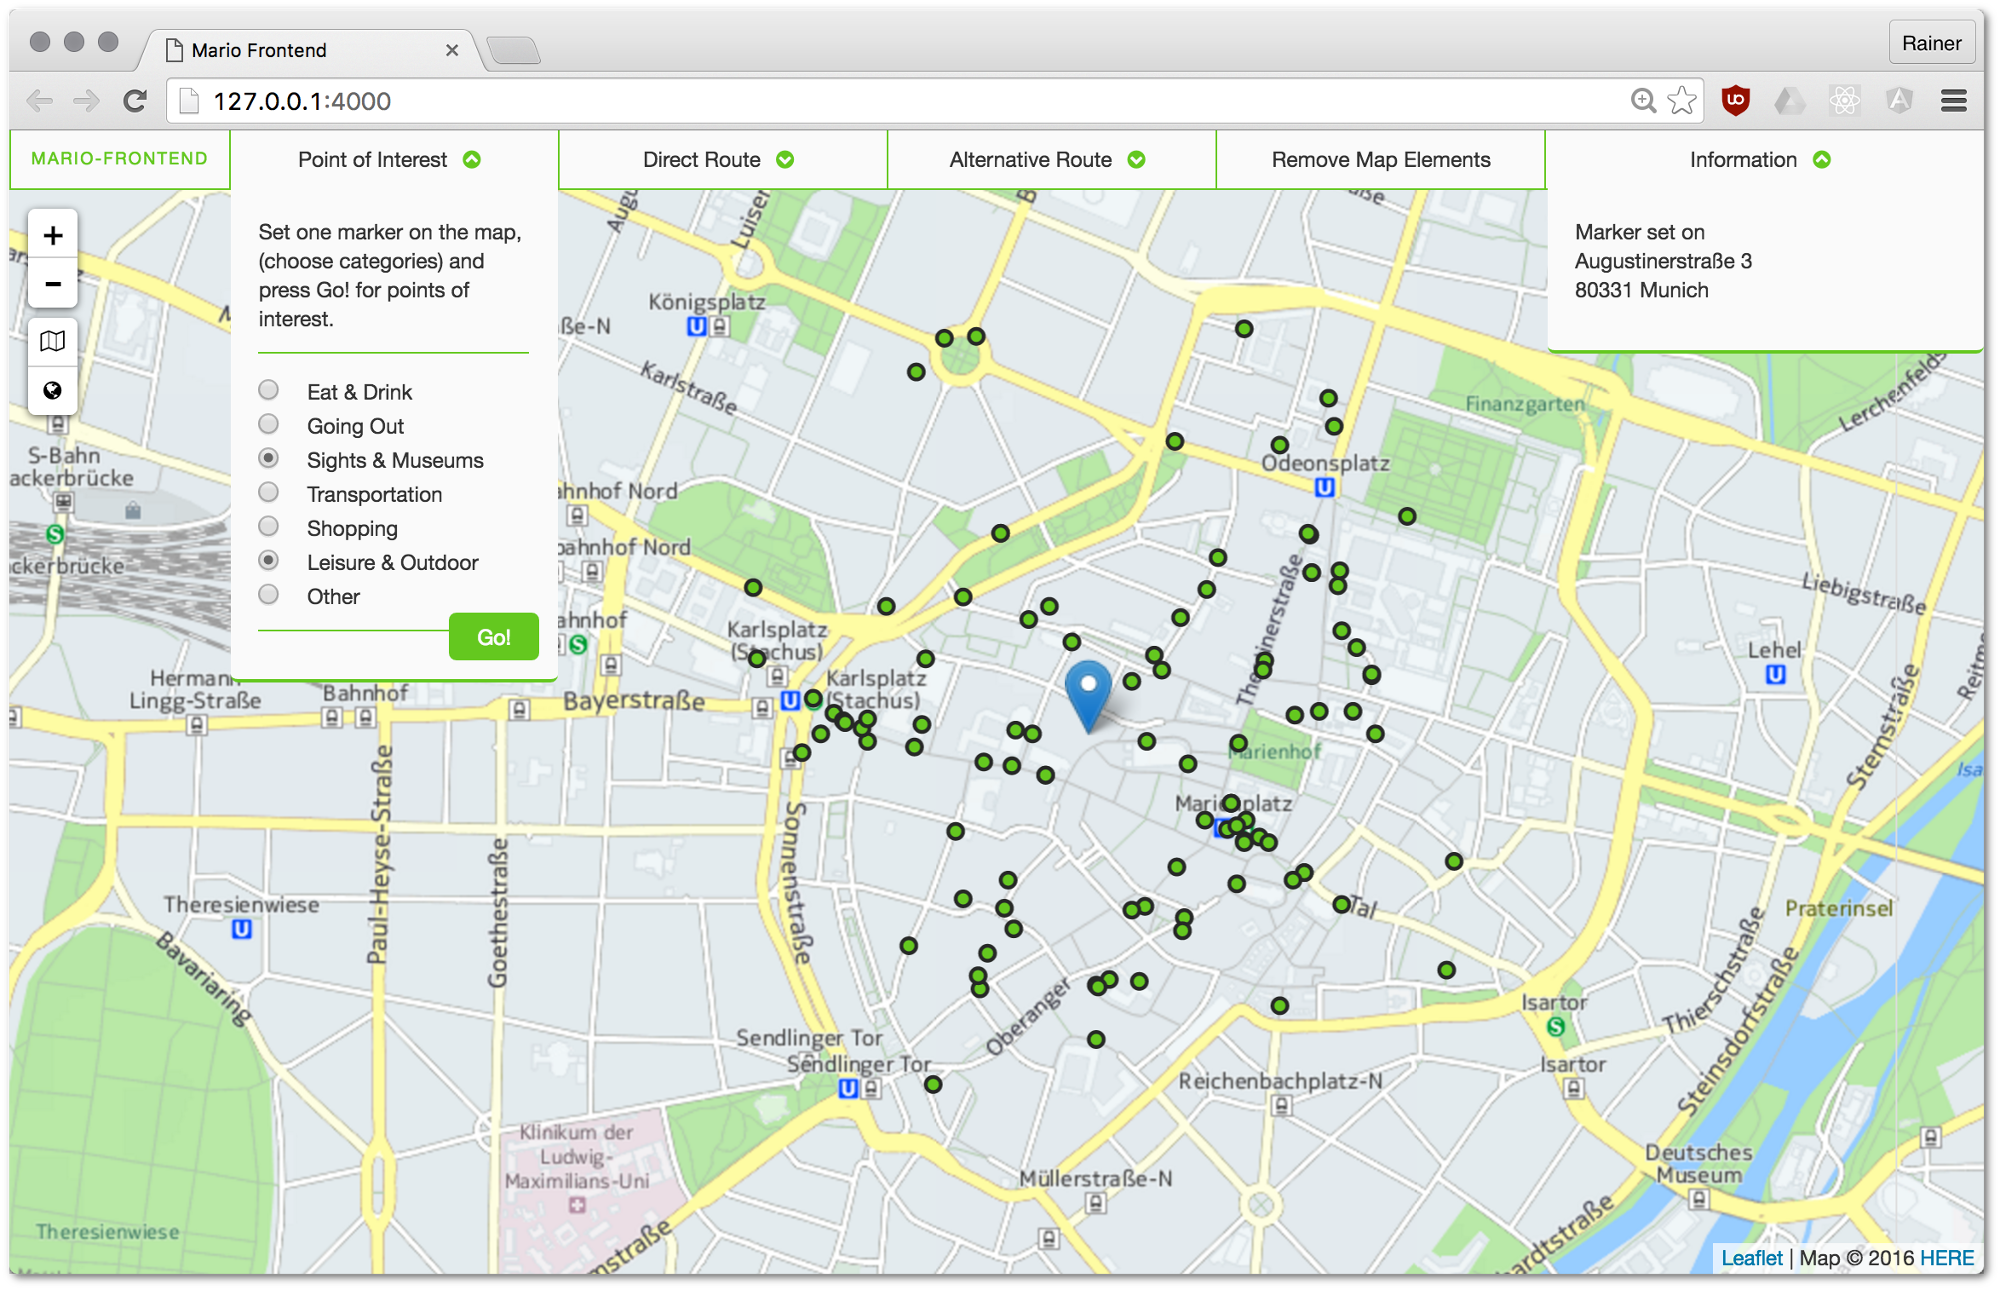
\includegraphics[width=0.95\columnwidth]{resources/DropdownPOI}
  \end{center}
  \caption{Front end with points of interest and open dropdown}
  \label{fig:DropdownPOI}
\end{figure}

A feature that was not originally intended to be implemented in the project, which was derived from the use case of displaying open parking spots at a given location, is the search for points of interest. Because there is no real data about parking spots available yet, this would have been implemented using simulation data from a different project at the DBS and would have included route calculations from origin point A to a parking spot near the destination point B \cite{Josse13}. As the display of parking spaces on a map has common elements with the displaying of any points of interest at a given location, the Point of Interest search was implemented (see figure \ref{fig:DropdownPOI}). This paragraph will describe the implementation of the feature and will identify technical difficulties and shortcomings.\medskip

To use this feature the user has to set one marker on the map to specify the location he is interested in. If two markers are set or a route is displayed both the route and the first marker are removed from the map once the Go! button is pressed. The user is able to select various categories like "Eat \& Drink", "Sights \& Museums", "Shopping" and many more and even combining more than one category, to choose which information he is interested in. The data than is displayed as small dots on the map with a popup opened by clicking on them, containing name, category and vicinity.

The technical integration of this feature was achieved by using one of the services of the HERE-API, the "Places" search. The request sent to the API has to include most importantly the location in latitude and longitude, the categories one is interested in, the search radius and a few other attributes mainly concerning the response type and format. If no category is selected by the user and consequently no selection is sent to the API, a list of points of interest in all categories is returned.

Up to twenty points of interest are included in one response. When more than twenty points of interest are available in the surrounding of the location a link to twenty more points is provided. This pattern of responses allow for up to five responses and therefore a maximum of 100 points of interest for one request. Leaving all categories unselected about 90 percent of the responses are associated with the "Eat \& Drink" category. Fortunately the response includes the corresponding category, the name of the point of interest and the physical address. Because of the included address this feature, for a short period of time, was evaluated for the in \ref{subsubsec:Geocoding Addresses} introduced reverse geocoding API but was dismissed for the lack of sufficient data in rural areas.\medskip

The performance of the "Places" endpoint was the most unreliable of the HERE services used in this project. In the majority of cases, the response time was around 300 ms for the first request to be answered and about 200 ms for additional points of interest via the above mentioned response pattern. In very few cases the performance was exceptional, receiving five responses in about one second and sometimes even less. On the other hand there were more exceptions leaving the user to wait for up to 15 seconds until all points of interest were rendered on the map.

Similar to the above mentioned route calculations to a parking spot one could implement an algorithm which calculates a route traversing a given number of points of interest on the way. Both topics will be discussed in chapter \ref{sec:recap}. 

%\____ Route Calculations

\subsubsection{Route Calculations v}
\label{subsubsec:Route Calculations}

\begin{figure}
  \begin{center}
    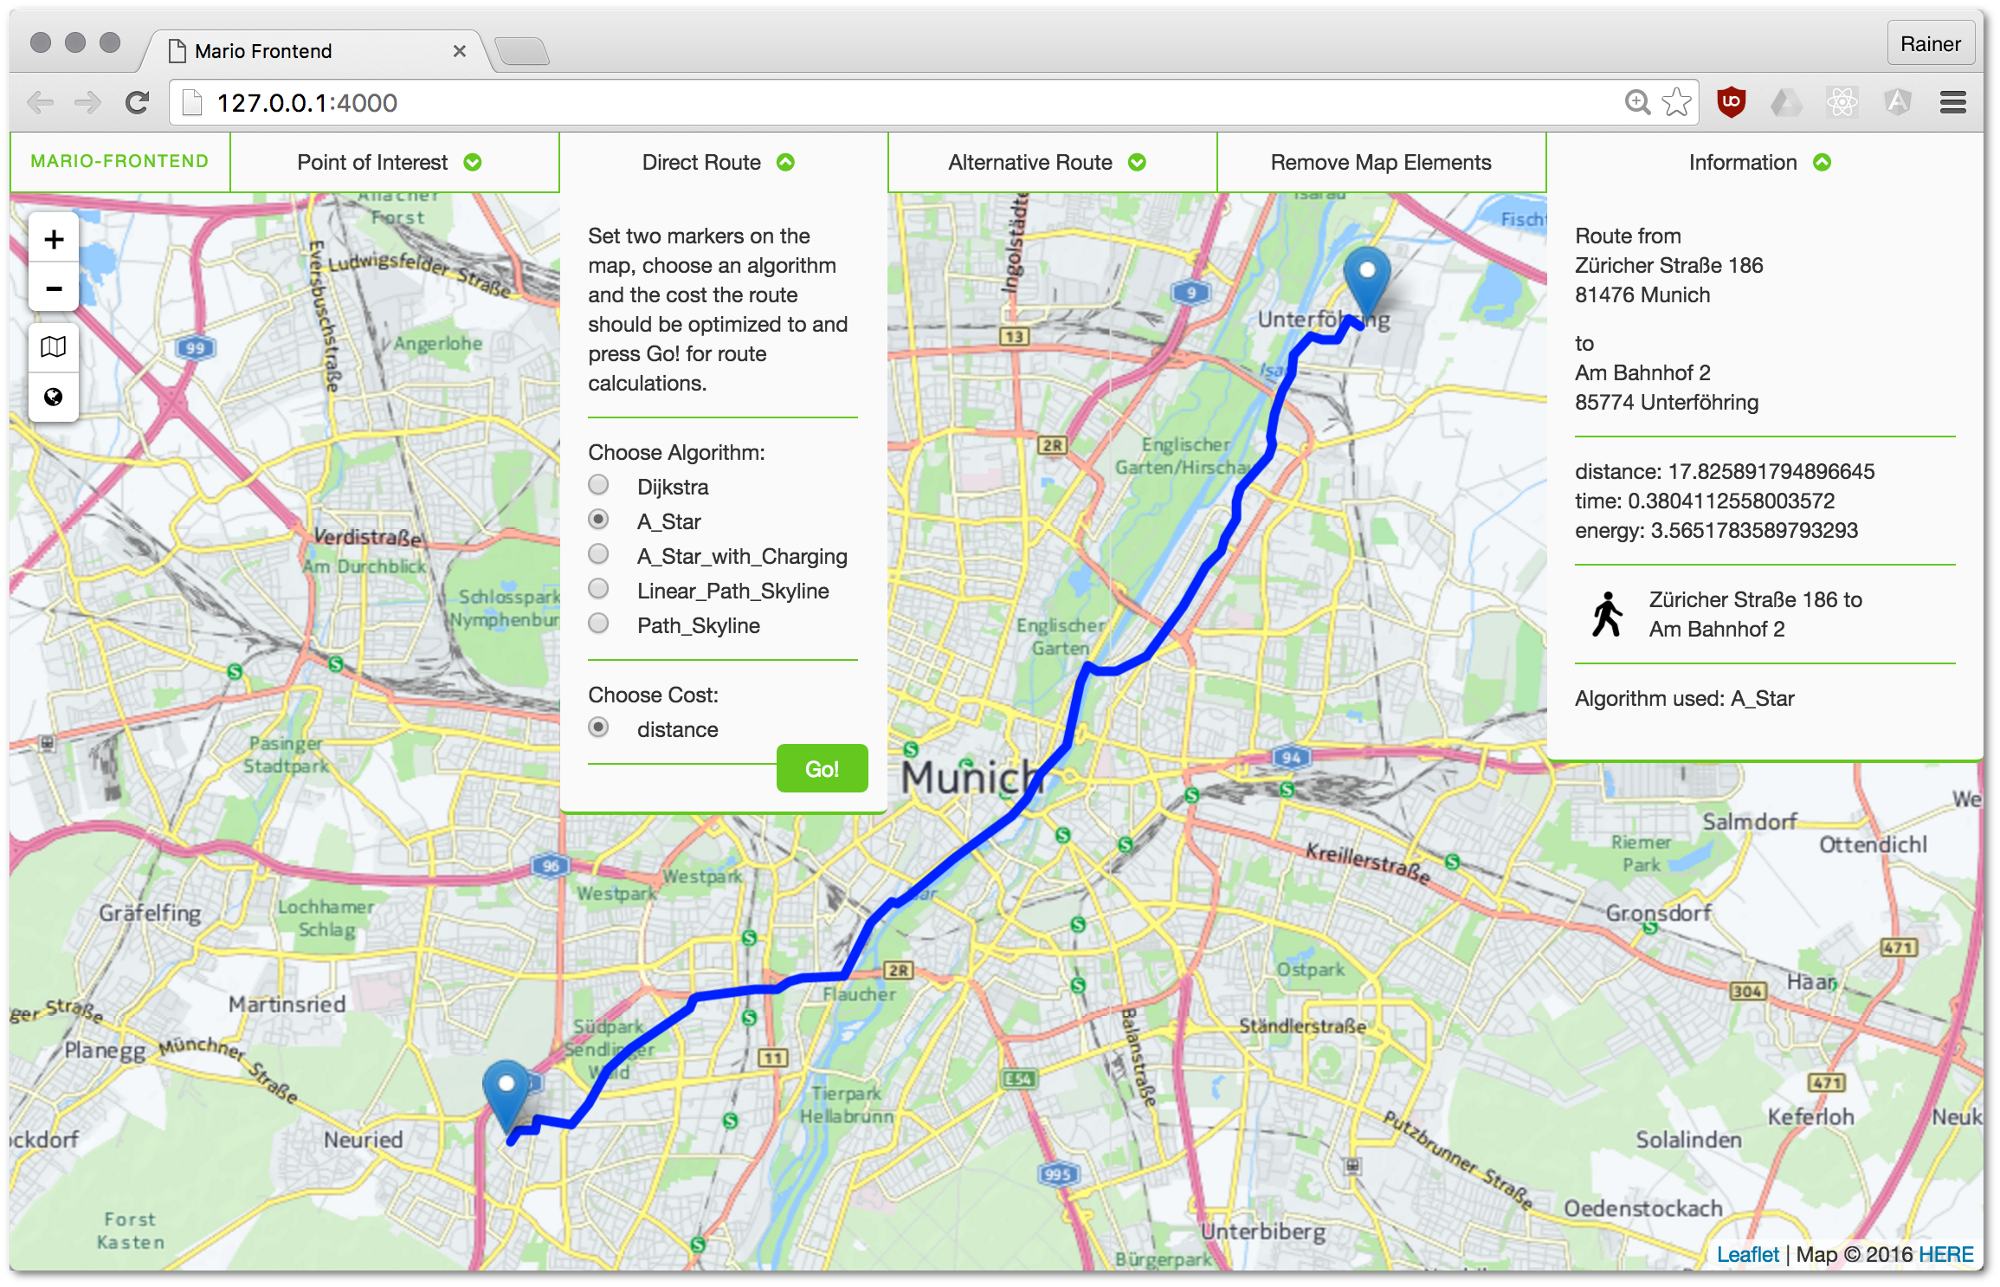
\includegraphics[width=0.95\columnwidth]{resources/DropdownAlgorithm}
  \end{center}
  \caption{Front end with calculated route and open dropdown}
  \label{fig:DropdownAlgorithm}
\end{figure}

The first of the two main features of this project is also the first feature to contact the in chapter \ref{sec:Description of the Backend} described server at DBS. It enables the user to request the calculation of a route between previously defined origin and destination from the server which is than displayed on the map with additional information available on the information panel. Via a dropdown the user can choose one of the in \ref{subsec:Backend Functionalities} defined algorithms and additionally allows the selection of the costs, which the route should be optimised to (see figure \ref{fig:DropdownAlgorithm}).\medskip

As new algorithms and new implementations are frequently introduced to the server by other projects, partly resulting from other students writing their theses at the DBS, a mechanism was needed to keep the information about algorithms up to date. For that reason an additional API call is triggered to the backend, requesting a file containing all implemented algorithms and their attributes. All new algorithms implemented on the server have to be included in that file for the front end to make them available for selection in the above mentioned dropdown.

Once the user has set two markers for origin and destination on the map and selected algorithm and costs, a request containing all information is send to the server for the calculation of the optimal route. The route is than sent back to the front end in GeoJson format and added to the map. Right after the route is added to the map a popup is bound to it containing the addresses of origin and destination. The route can be highlighted on hover over the route itself or the route description in the information panel. Both features are especially helpful for intermodal route calculations introduced in \ref{subsubsec:Intermodal Route Calculations}.\medskip

\begin{figure}
  \begin{center}
    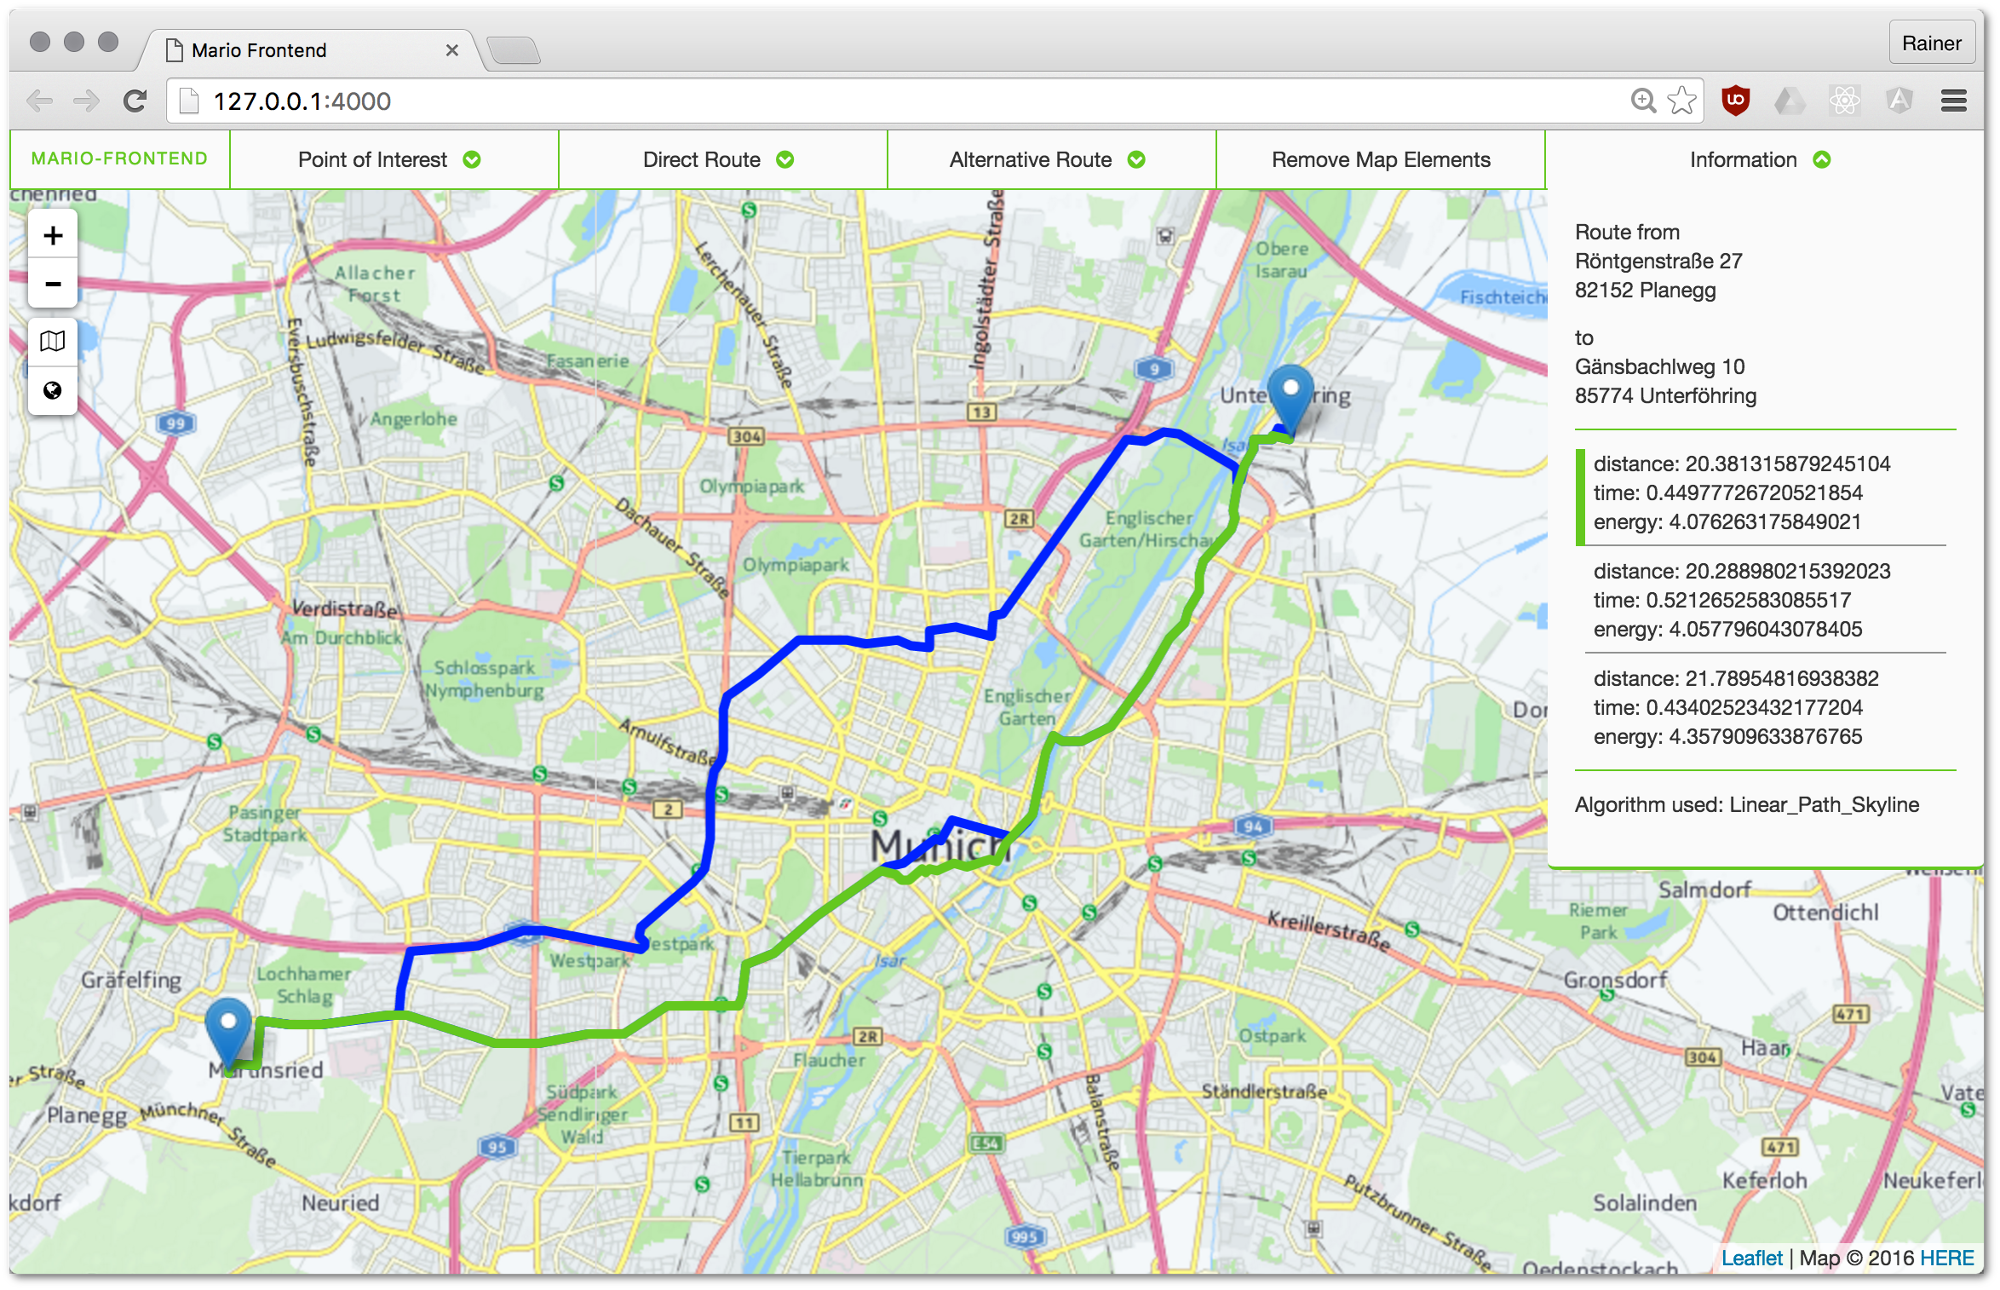
\includegraphics[width=0.95\columnwidth]{resources/HighlightingSkyline}
  \end{center}
  \caption{Front end with highlighted route}
  \label{fig:HighlightingSkyline}
\end{figure}

At this moment, there are two cases receiving different treatment than described above. On of them is the algorithm called a-star-with-charging which was implemented for electrical vehicles, as described in \ref{subsec:Backend Functionalities}. The response to a request with this algorithm selected contains a route with a charging station on the way and a point, where the station is located. The route is added as above and the charging station is added as a special marker to the map.

The second case comprises all algorithms from the skyline family. As delineated in \ref{subsec:Backend Functionalities} the skyline algorithms are able to optimise route calculations to more than one cost. That's why the user is able to select more than one or even all of the available costs in the direct route dropdown. The server returns a collection of routes in geojson format with the associated costs attached to the features. Adding the costs to the information panel of the front end instead of the addresses of the origin and destination allows the user to compare different routes in regard to their efficiency. The above mentioned route highlighting helps to differentiate between the displayed routes (see figure \ref{fig:HighlightingSkyline}).

One additional feature would have been implemented for further analysis of the algorithms, if time would have allowed it. The displaying of visited nodes in the graph to better understand how the algorithms work will be described in chapter \ref{sec:recap}.

%\____ Intermodal Route Calculations
\clearpage
\subsubsection{Intermodal Route Calculations}
\label{subsubsec:Intermodal Route Calculations}

\begin{figure}
  \begin{center}
    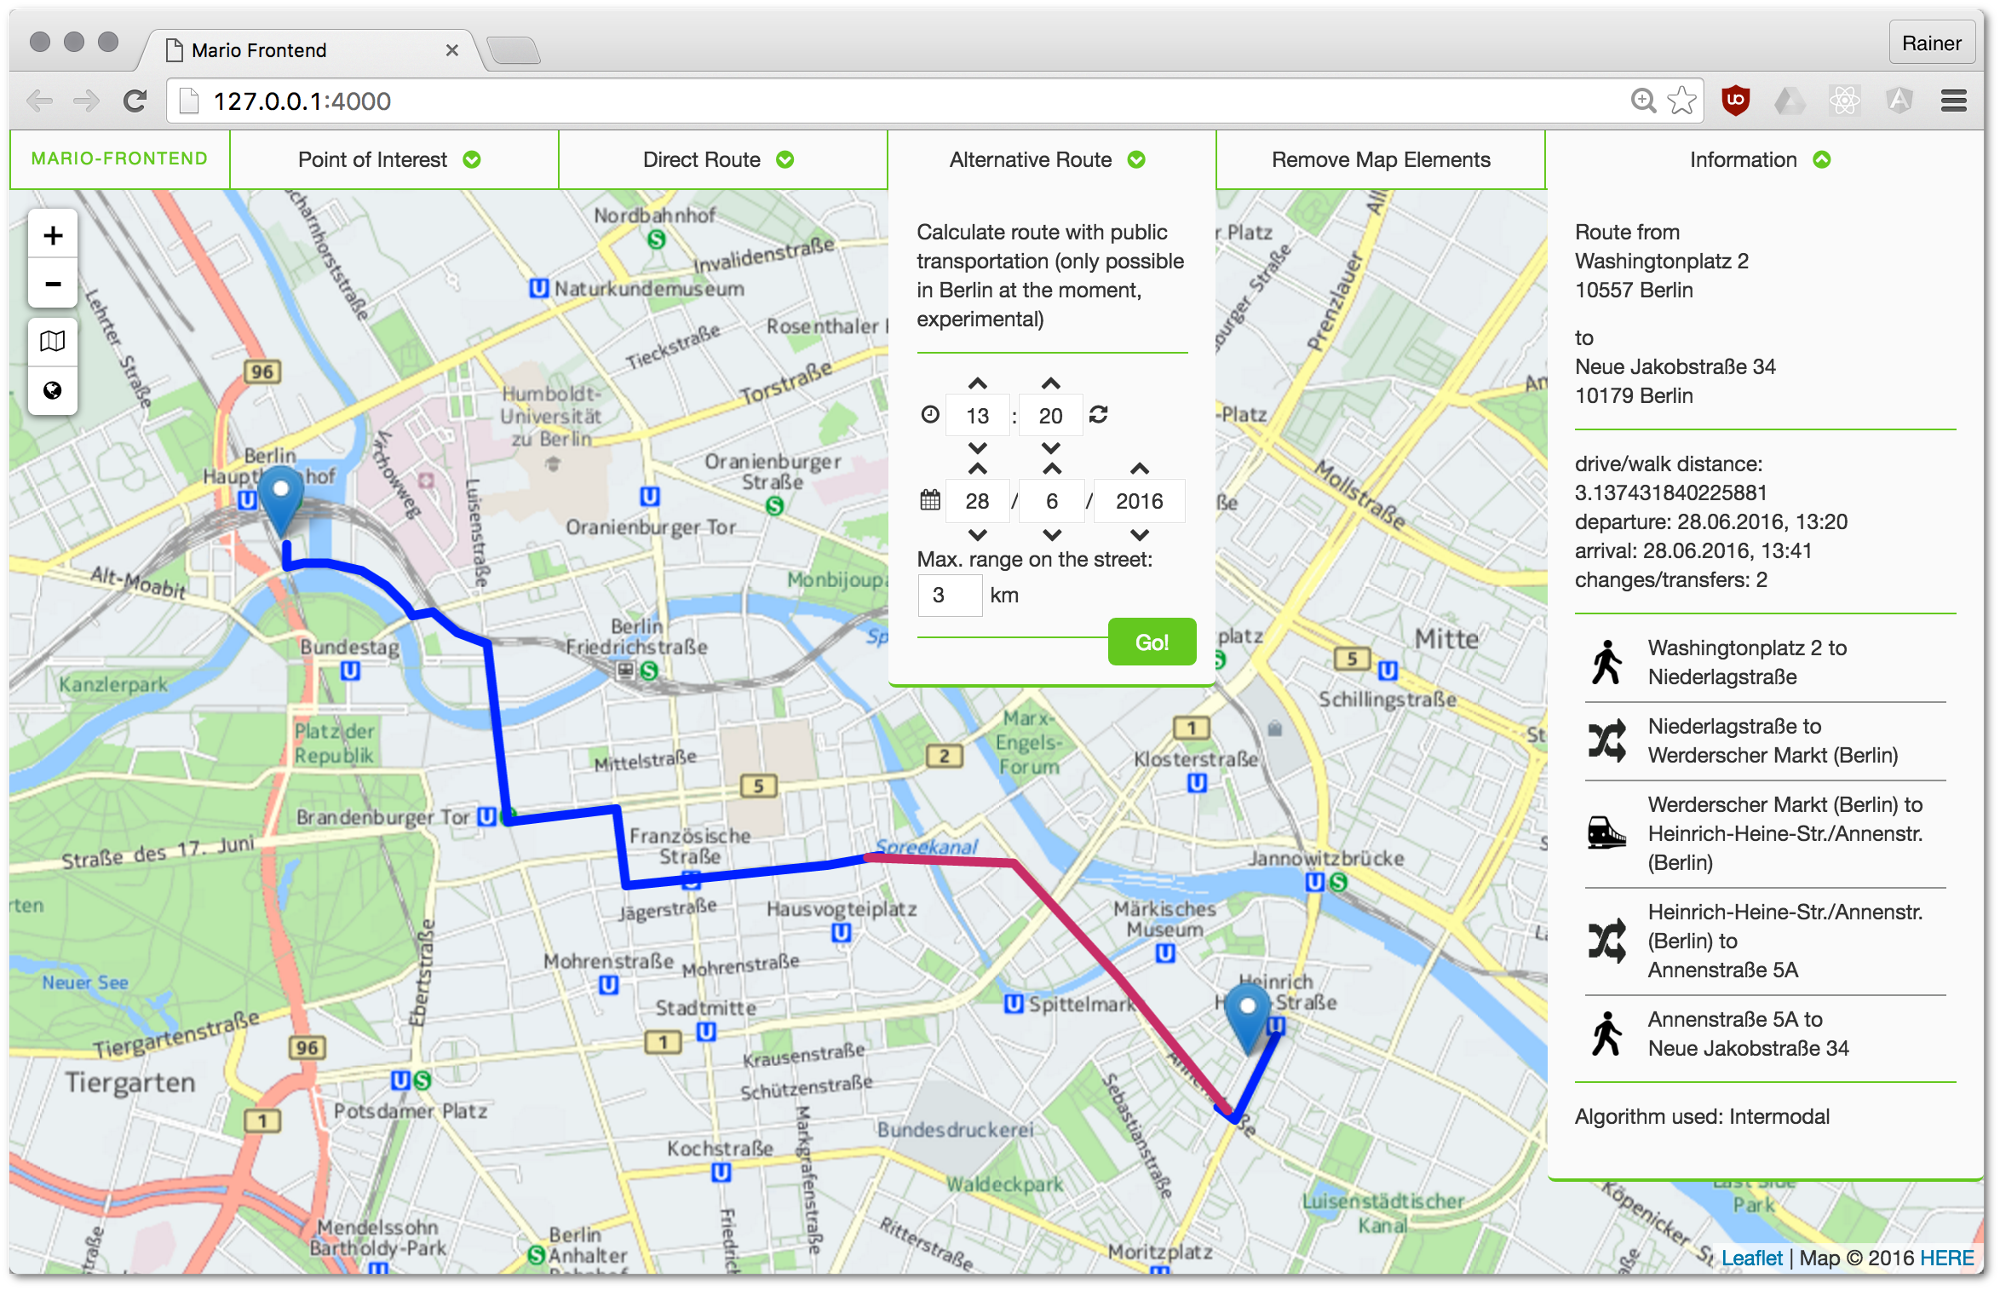
\includegraphics[width=0.95\columnwidth]{resources/DropdownIntermodal}
  \end{center}
  \caption{Front end with intermodal route and open dropdown}
  \label{fig:DropdownIntermodal}
\end{figure}

The second main feature is the calculation of intermodal routes using public transportation such as trains and busses. This service is experimental and currently only available for the Berlin metro area. Similar to route calculations in \ref{subsubsec:Route Calculations} the user has to set two markers on the map for origin and destination. Because the intermodal route calculations are executed using an implementation of Dijkstra's algorithm optimised to time as cost, the user is neither able select algorithms nor costs. Additional to origin and destination the user has to specify the time of departure and the range in km he is willing to go by foot, bike or car. The departure time is automatically set to the current system time on page load and is updated only on page refresh to allow the user to check varieties of the route by changing the range parameter.\medskip

The response is a single route divided into at least five segments including walk or drive segments, train or bus rides and the changes of the mode of transportation. For easier identification of the mode of transportation and understanding of the instructions segments using public transportation are added in red and representative icons are added to the respective segment on the information panel (see figure \ref{fig:DropdownIntermodal}). The user also receives the walking distance, departure and arrival time and the number of changes, which are also displayed on the information panel.

The performance of this API endpoint (see section \ref{subsec:Rest API}) is rather uncertain and fluctuates between 400 ms and 30 seconds. This, of course, is not acceptable for any kind of client application and has to be addressed in further work on the back end implementation. Additionally, if the server is not able to find any route corresponding to the users input, no answer is sent to the client application at all, rendering it unable to determine whether the server is slow or no route was found.

Paragraph about wrong instructions (too long public lines)\medskip

Albeit the from the German Bundestag unveiled action plan to implement the open data charter established by the G7 countries in September 2014 with the goal to make all government data and all data with public interest accessible to everyone, not many agencies and companies follow these rules. Although it is highly interesting for the public, one of the only providers of public transportation data is the state Berlin, which offers an API to access departure times, route information, etc while also allowing the download of bulk data sets. The provided data follows the General Transit Feed Specification (GTFS).

For more control over the results and reproductivity the bulk download method was chosen for this project leaving the maintainer to manually download the data from the official source and upload it to the server at the DBS. Because of the enormous file size only two month of data can be held on the servers memory at any given time. This is also an issue that needs to be addressed in future work on the back end implementation.

%\____ Geocoding Addresses

\subsubsection{Geocoding Addresses v}
\label{subsubsec:Geocoding Addresses}

\begin{figure}
  \begin{center}
    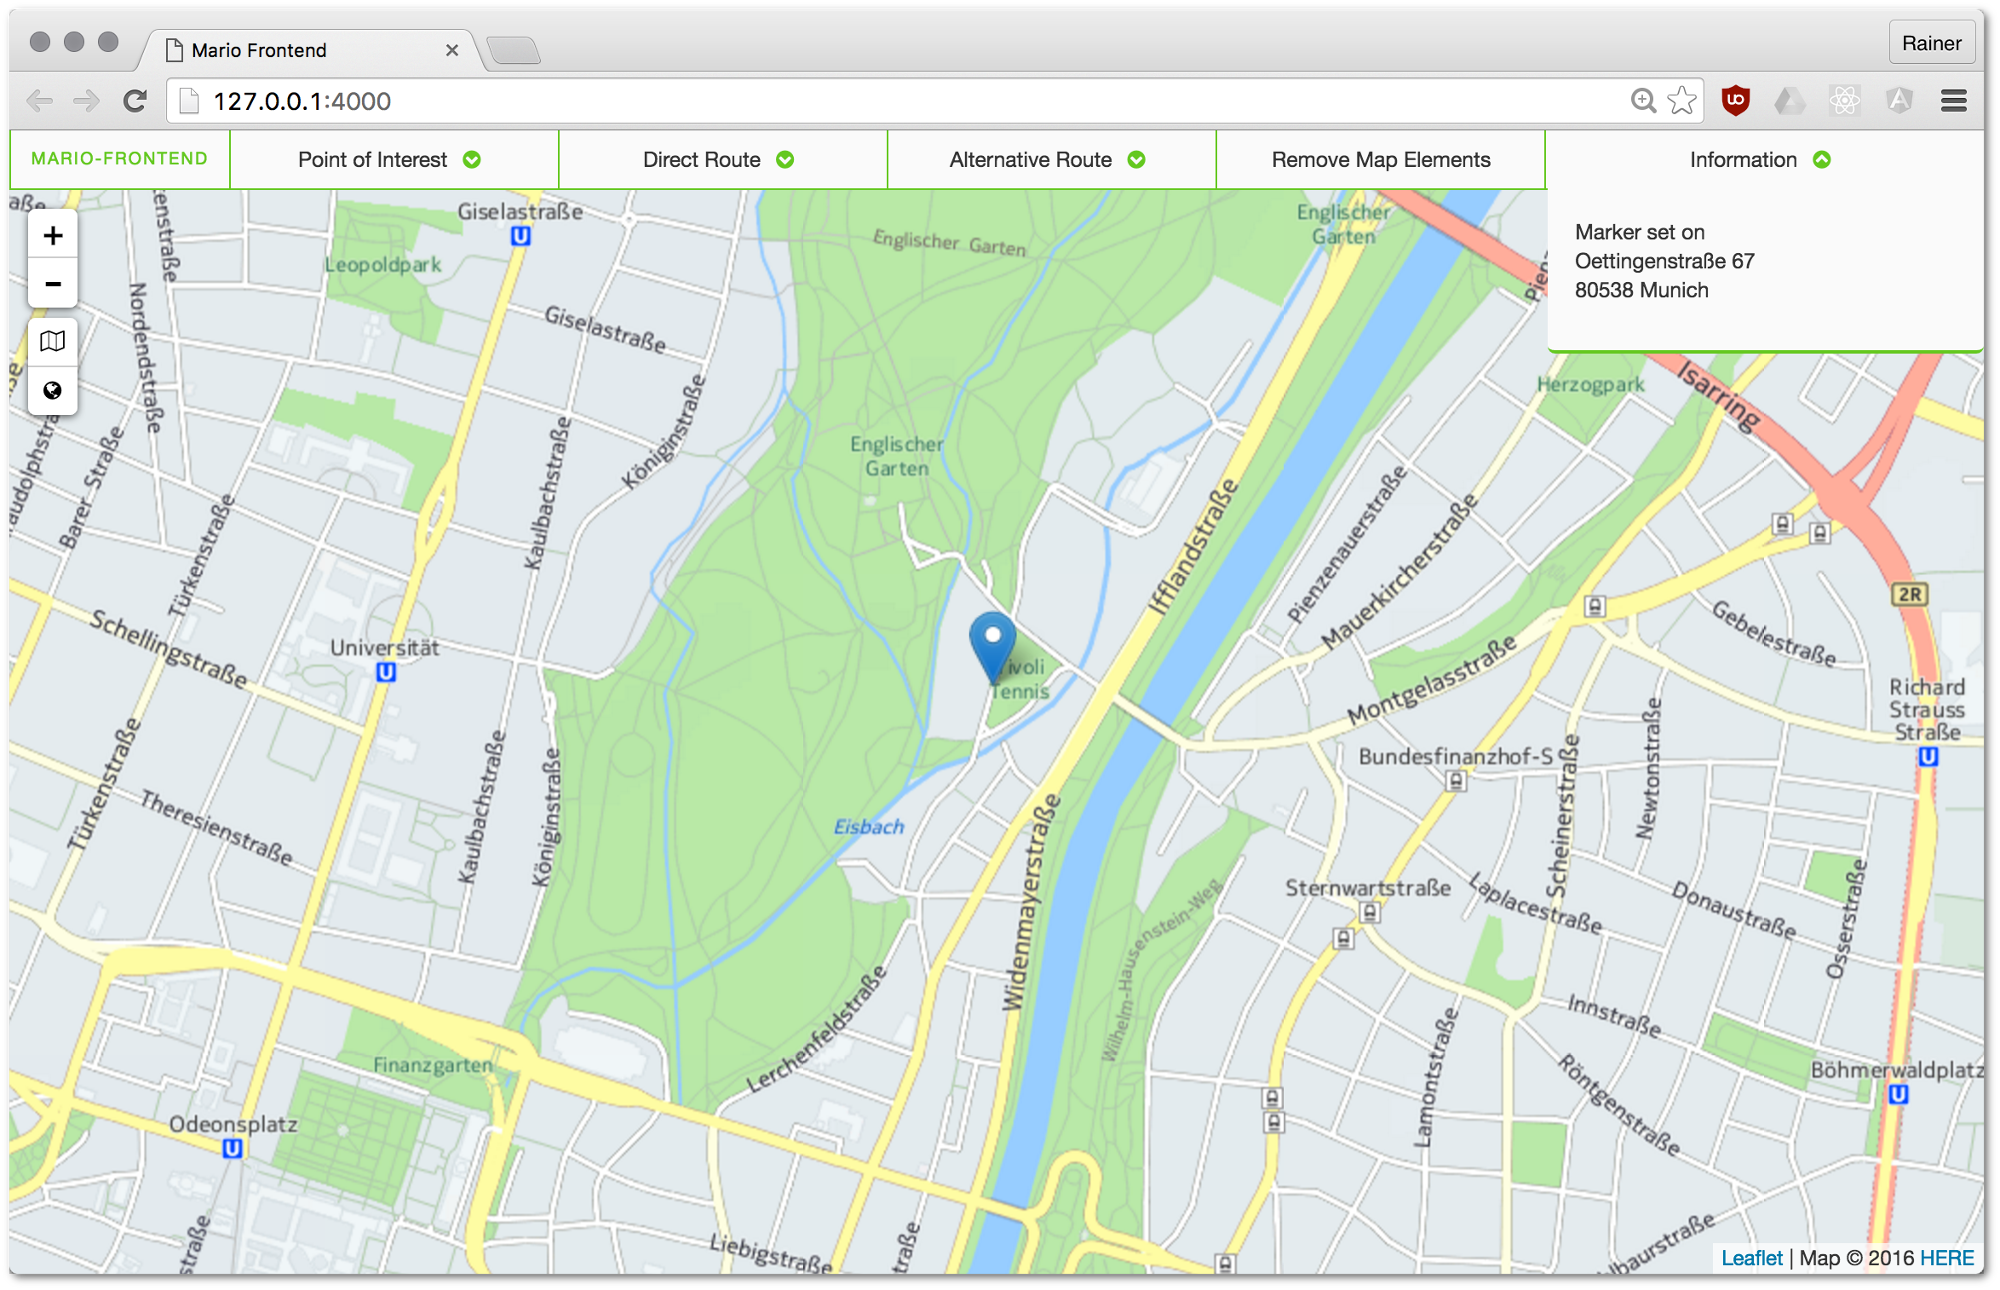
\includegraphics[width=0.95\columnwidth]{resources/GeocodingAddress}
  \end{center}
  \caption{Front end with marker and displayed address}
  \label{fig:GeocodingAddress}
\end{figure}

For better understanding of route descriptions and set markers a reverse geocoding API was integrated into the project to translate latitude and longitude data into physical addresses (see figure \ref{fig:GeocodingAddress}). This paragraph will outline the implementation of this feature, describe the usage of the HERE-API as reverse geocoding service, compare it to other geocoding services and highlight key features and problems encountered in the development process.\medskip

When a marker is set on the map by clicking, two processes are set into motion. Firstly, the image of the marker is loaded and pinned to the location the user clicked on and secondly, the position of the click is saved to the scope in latitude and longitude. In the bootstrapping phase of the application, that is the loading of the core functionality of AngularJS into the HTML document, a watcher is defined to listen to changes in the marker directory of the scope. For every change in that directory the new or updated location of a marker is sent to the reverse geocoding API and the new address is sent back to the application, which is than saved to the scope for display. The two way data binding of AngularJS comes in really handy in this instance because otherwise a very complex and complicated process would have to be implemented to generate that functionality. 

This feature increases its value in the in \ref{subsubsec:Intermodal Route Calculations} introduced intermodal route calculations. As you know, the route is calculated to include public transportation which implies that the route is split into segments. Each segment has an origin and a destination and for every one of these points the physical address is requested from the reverse geocoding API and displayed as a from-to statement in the route information panel of the application.\medskip

The basics of the HERE-API are described in Chapter \ref{subsec:HERE API} so only the specific properties of the reverse geocoding API will be illustrated in this section. As all other parts of the HERE conglomeration the geocoding API is only well documented to a certain extend, for the documentation is so bulky that one is better off just implementing and testing it. The error descriptions and actual data responses are far better to understand the workings of the API than just reading the documentation. For historic reasons and to satisfy a similar data structure in all HERE APIs the response data to a reverse geocoding request is strictly hierarchical and multilayered. Especially in this case alternatives to the HERE API such as Nominatim, maintained by the OpenStreetMap Foundation and OpenCage Geocoder run by the OpenCage Data Ltd. would have been preferable but both couldn't be used because of the strict limitation to one request per second.\medskip

Implementing the API one can define the mode of the request. For translating latitude and longitude intro physical addresses the modes "retrieve addresses" and "track position" are applicable, although the second one is a bit alienated for that purpose. "Retrieve addresses" returns a by the developer specified number of addresses which are ordered by the distance to the requested location. For an inexplicable reason in some cases the state or city is returned as nearest address without any information about street or house number. Accordingly the results had to be filtered to satisfy the need for a correct address. "Track position" is intended to be used for mobile navigation as it incorporates the direction in which the user is moving for the calculations usually returns the better results because it snaps to the nearest address it can find and returns just that. Unfortunately this mode is not reliable in more remote areas and returns no address at all in some cases. 

For this project the more dependable mode "retrieve addresses" was chosen and logic was implemented to select the best quality address from the five responses. The "match-level" parameter associated with each address was helpful but not reliable because the above mentioned addresses, only containing city or state, sometimes also have the highest match level possible, what is probably a wrong implementation on the providers side. Again, other geocoding APIs would have been preferable but couldn't be used because of rate limitations. Notable is the fast response time of the API which almost never exceeded 100 ms and was thus on average two times faster than Nominatim and almost four times faster than OpenCage Geocoder.

%\begin{verbatim}
%Response: {
%  MetaInfo{...}
%  View: [{
%    0: {
%      Result: [{
%        0: {
%          Distance: 16.1,
%          Location: {
%            Address: {
%              Label: "Karlstra�e 37, 80333 Munich, Germany",
%              ...
%            }
%          }
%        }
%      }]
%    }
%  }]
%}
%\end{verbatim}

%\____ Simulation

\subsubsection{Simulation v}
\label{subsubsec:Simulation}

\begin{figure}
  \begin{center}
    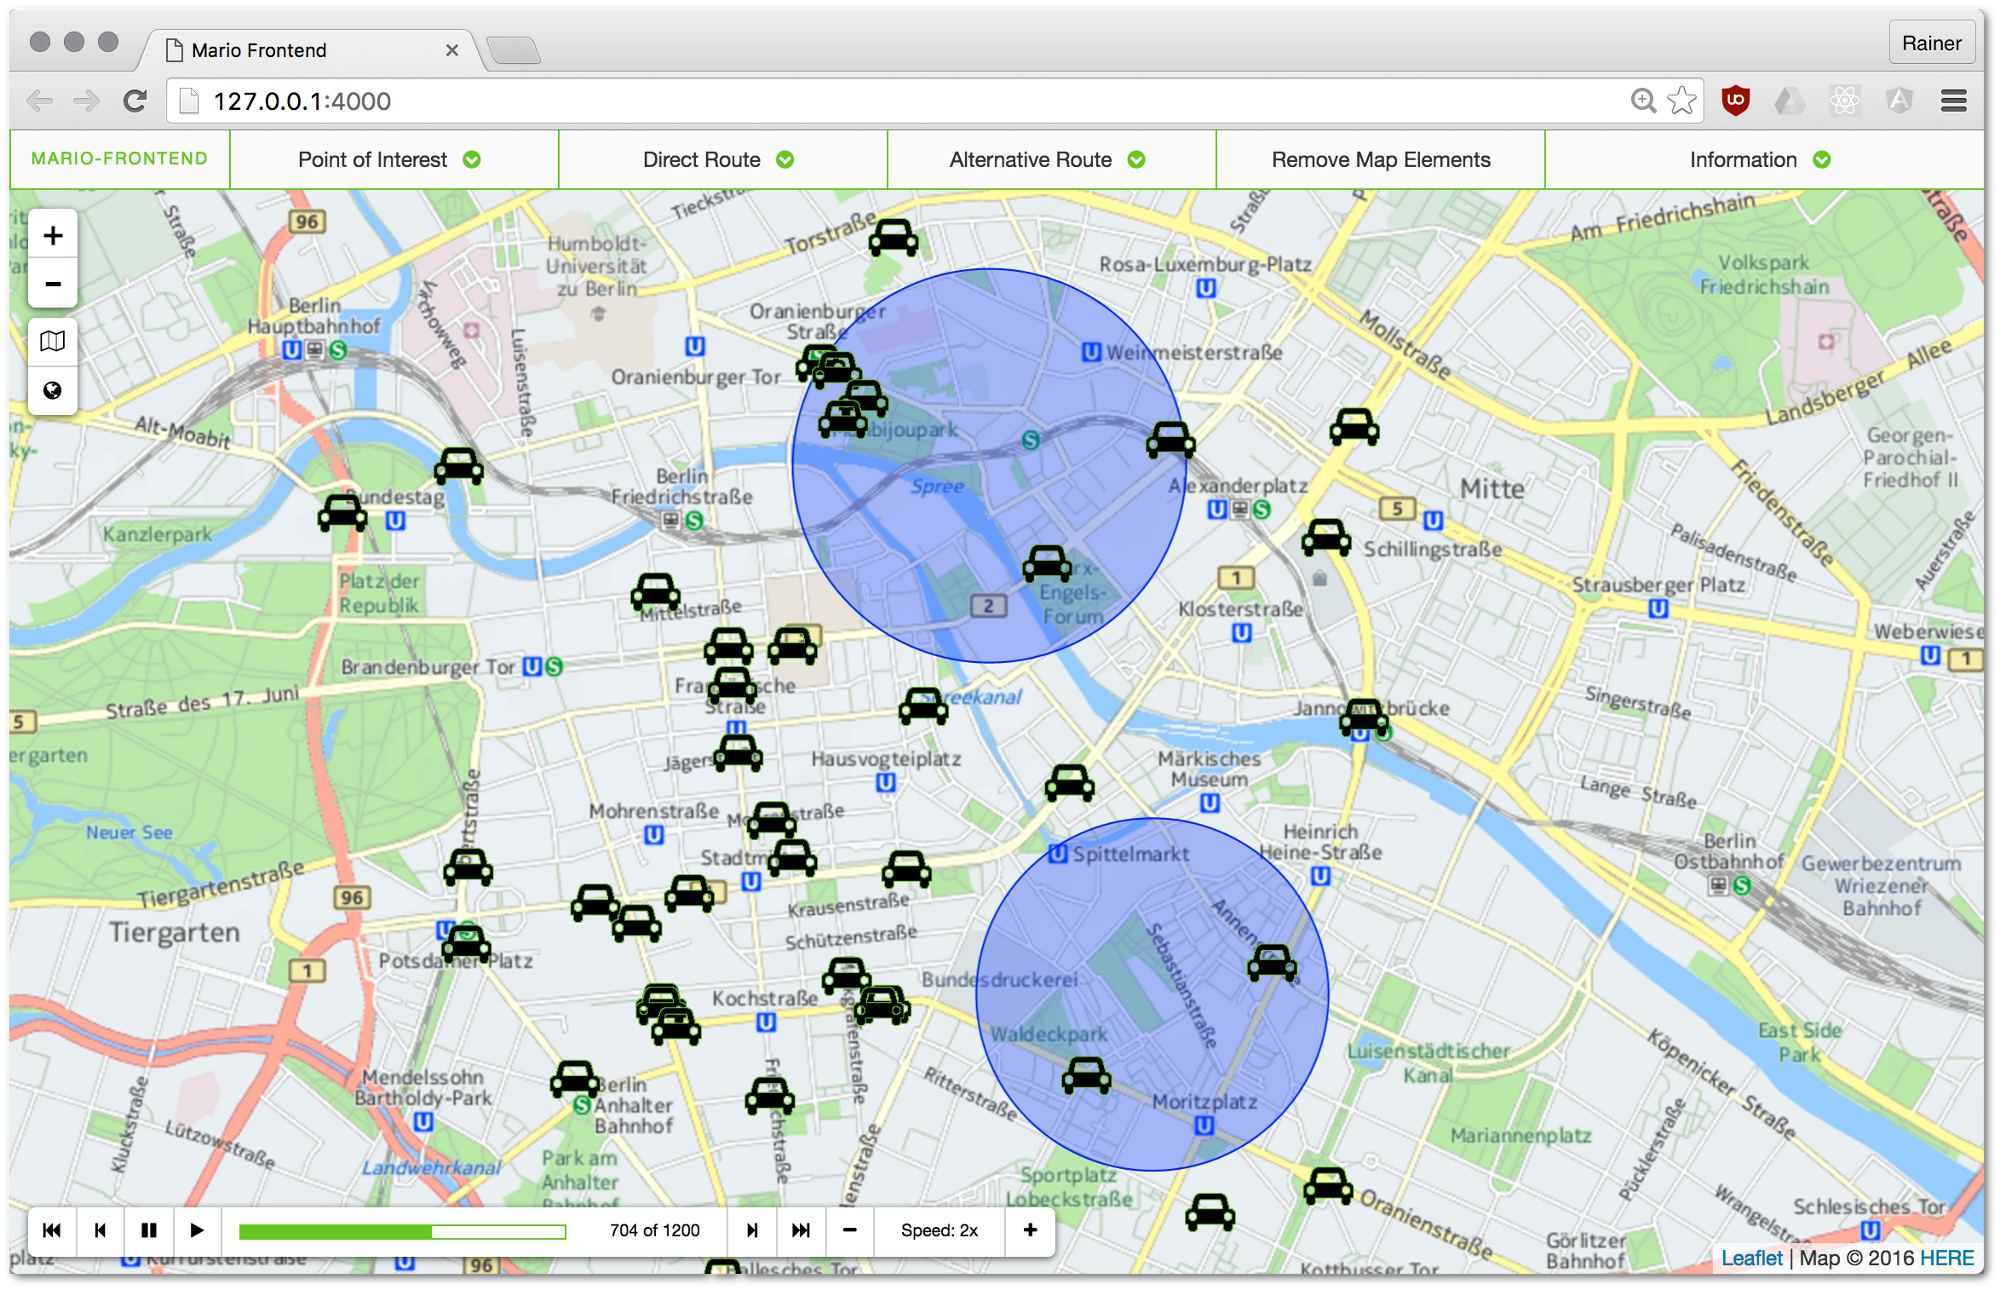
\includegraphics[width=0.95\columnwidth]{resources/Simulation}
  \end{center}
  \caption{Front end with running simulation of cars and weather}
  \label{fig:Simulation}
\end{figure}

Algorithms and methodologies developed at the DBS have the tendency to be abstract and hard to grasp. This is especially true for simulations with high data output like the one integrated in this project. Jenny Lauterbach develops and implements a system to simulate vehicles driving through a street network and how they are influenced by external factors, such as heavy weather simulated as circular storms moving across a simulation area. This is an ongoing project at DBS under the supervision of PD Dr. Matthias Schubert. The next few paragraphs will not describe the developed system but the implementation of simulation data into this project's front end.\medskip

As a simulation of this kind adds time as an additional dimension to this project, a control panel had to be implemented to navigate through the up to 3600 states that where generated by the above mentioned system. This panel (see bottom left corner of figure \ref{fig:Simulation}) includes play and pause buttons, step forward and backward and jumps forward and backward. Additionally the user is able to jump to a specific part of the simulation by clicking on the control bar. Later in the project the simulation speed control was introduced to specify the play-back speed between 1/4 and four times the normal speed.\medskip

Currently the user is not able to select an area for the simulation as there is no web service or API provided by Jenny Lauterbach's project. The temporary workaround is to generate simulation files, converting them to GeoJson, adding them manually to the project and later load them from the web server, the font end is hosted at. At this point this workaround is probably the only way to display simulation data produced by the system because generating the file and downloading it to the application would take more time than one would be willing to wait. Furthermore the output data is not in GeoJson format and has to be converted manually.

The GeoJson file is structured into cars and storms which are grouped as GeoJson-Features according to their timestamp. Each vehicle has a position in latitude and longitude associated to it which makes it easy to add them as markers to the map. The icon of a car is used as marker image to clarify what they symbolise. Storms on the other hand have to be treated otherwise since they have a spatial component. These are added as so called circular paths with the radius provided in the file. On first load of the simulation data the first state of cars and storms, identified by the timestamp of 0, are added to the map.

The animation of moving elements is essentially achieved by removing all vehicles and storms and adding the ones of the next step. These, again, are identified by the timestamp associated with the data. On normal speed, the scene is repainted about twenty times per second and can be slowed down to five and speedup to about eighty repaints per second. In a few instances a slight flickering of the storms was noticed but unfortunately it was neither possible to detect the source of the error nor to determine the specific system setup the led to it. 

%\____ Legal Basis and Copyright of Map Material

\subsection{Legal Basis and Copyright}

%\_____________________________________________________________________

%\cleardoublepage
%\section{User Experience and Interface Design}
%\label{sec:User Experience}

%\____ User Interface Design

%\subsection{User Interface Design}
%\label{User Interface Design}

%\____ User Experience

%\subsection{User Experience}
%\label{User Experience}

%\_____________________________________________________________________

\cleardoublepage
\section{Modularity}
\label{sec:Modularity}

\subsection{Modularity in Web Development}
\label{subsec:Modularity in Web Development}

\subsection{Modularity in the MARiO Project}
\label{subsec:Modularity in the MARiO Project}

%\_____________________________________________________________________

\cleardoublepage
\section{Recapitulation and Future Work}
\label{sec:recap}

- parking spots and route to points of interest as proposed in \cite{Josse15}\medskip

- display of visited nodes

%______________________________________________________________________

\cleardoublepage
\begin{thebibliography}{99}

%Citations in Harvard Style

%\bibitem{Ivory01}

%  M.\ Y.\ Ivory, M.\ Hearts:
%  \href{http://www.ischool.washington.edu/myivory/thesis/thesis.pdf}{%
%    An Empirical Foundation for Automated Web Interface Evaluation}.
%  Ph.D. thesis, University of California at Berkeley, 2001

\bibitem{Crickard14}
  Crickard III, P., 2014, August:
  \textit{Leaflet.js Essentials}.
  Packt Publishing Ltd.
  
\bibitem{MARiO11}
  Graf, F., Kriegel, H.P., Renz, M. and Schubert, M., 2011, August:
  MARiO: multi-attribute routing in open street map.
  In \textit{International Symposium on Spatial and Temporal Databases} (pp. 486-490).
  Springer Berlin Heidelberg.

\bibitem{Josse13}
  Joss�, G., Schubert, M. and Kriegel, H.P., 2013, November: 
  Probabilistic parking queries using aging functions. 
  In \textit{Proceedings of the 21st ACM SIGSPATIAL International Conference on Advances in Geographic Information Systems} (pp. 452-455).
  ACM.

\bibitem{Josse15}
  Joss�, G., Schmid, K.A., Z�fle, A., Skoumas, G., Schubert, M. and Pfoser, D., 2015, August:
  Tourismo: A User-Preference Tourist Trip Search Engine. 
  In \textit{International Symposium on Spatial and Temporal Databases} (pp. 514-519).
  Springer International Publishing.


\clearpage
\hspace{-\leftmargin}{\Large\bfseries Web-Referenzen} % W�ster Hack %-|

\bibitem{Agafonkin15}
  Agafonkin, V., 2015, May:
  \textit{Leaflet story in 13 minutes}, 
  \url{https://youtu.be/NLbyHffKQuU}, accessed July 18, 2016

\bibitem{ECMA}
  ECMA, 2016, June:
  \textit{Standard ECMA-262 ECMAScript Language Specification, 7th edition},
  \url{http://www.ecma-international.org/publications/files/ECMA-ST/ECMA-262.pdf}, accessed July 18, 2016
  
\bibitem{MacWright13}
  MacWright, T., 2013, April: 
  \textit{Announcing MapBox.js 1.0 with Leaflet},
  \url{https://www.mapbox.com/blog/mapbox-js-with-leaflet/}, accessed July 18, 2016

\bibitem{WFS}
  OGC, 2014, July:
  \textit{OGC Web Feature Service 2.0 Interface Standard},
  \url{http://www.opengeospatial.org/standards/wfs}, accessed July 18, 2016

\bibitem{WMS}
  OGC, 2006, March:
  \textit{OpenGIS Web Map Server Implementation Specification},
  \url{http://www.opengeospatial.org/standards/wms}, accessed July 18, 2016

\end{thebibliography}

\end{document}
